	\newpage
\section{Implementacja}		%4
%Wkleić szkielet kodu, wraz z komentarzami. Opisać zmienne, struktury do czego służą. Opisać procedury, metody co wykonują. Opisać nowe zdefiniowane klasy. Opisać dziedziczenie. Opisać nowo utworzone pliki za co odpowiadają.
\subsection{Pierwsze kroki}
\textit
{
	Po stworzeniu projektu poznawaliśmy strukturę oraz działanie aplikacji próbując modyfikować istniejące już klasy. Po zapoznaniu się z podstawami realizowaliśmy dalsze tutoriale aby swobodnie pracować w środowisku Xamarin'a.
}

\subsection{Modyfikacja menu}

\textit
{
	Pierwszym zadaniem było ustalenie szaty graficznej, widoku podstawowego z przyciskiem oraz menu. Aby to zrobić należało wykonać następujące czynności:\\\\
	-Dopisać odpowiednie właściwości do kodu XML, takie jak background color, font-size, padding, textcolor itp., aby wystylizować układ widoku. Na rysunku 4.1 znajduje się fragment wprowadzonych modyfikacji.\\
	\begin{figure}[!htb]
		\begin{center}
			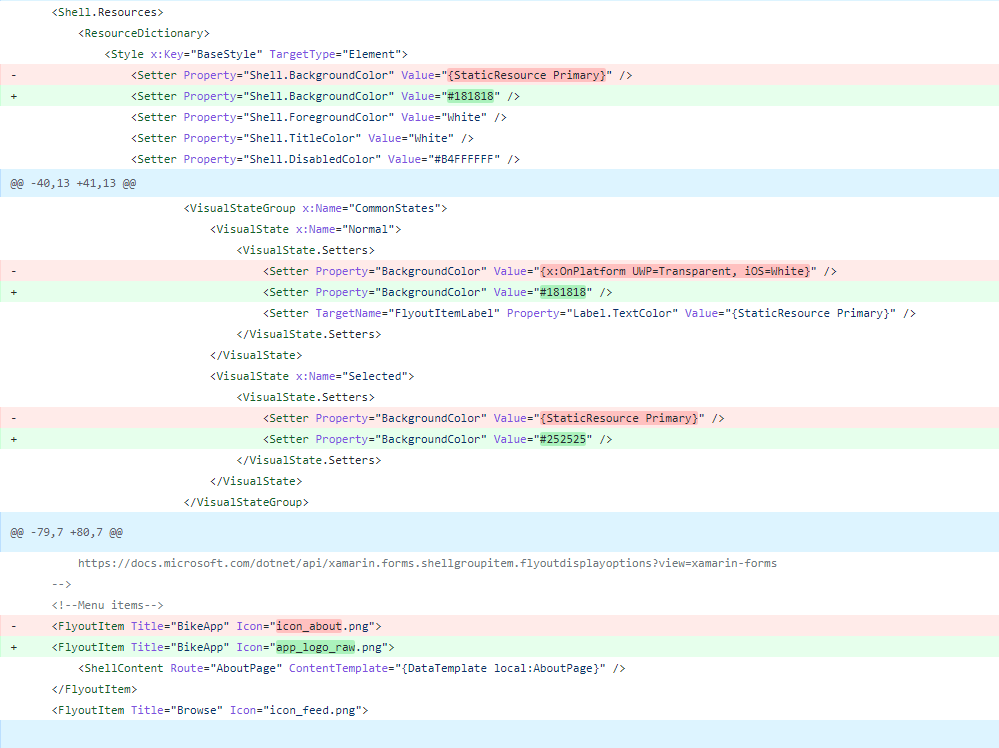
\includegraphics[width=15cm]{rys/gitchanges1.png}
			\caption{Dodanie właściwości stylujących widok}
			\label{rys:Dodanie właściwości stylujących widok}
		\end{center}
	\end{figure}
}

\newpage
\textit
{
	-Stworzyć widok główny na podstawie języka XML oraz metody w języku C\# informującej o kliknięciu w przycisk (zgodnie z rysunkiem 4.2).\\
	\begin{figure}[!htb]
		\begin{center}
			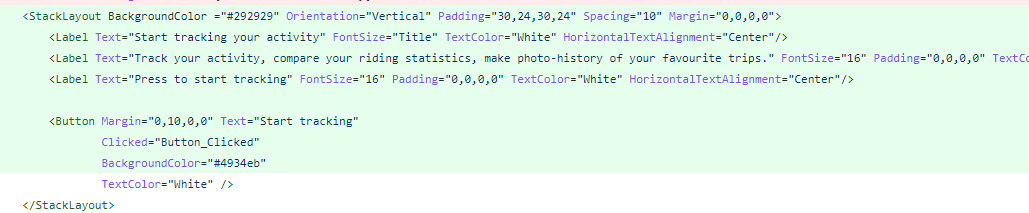
\includegraphics[width=15cm]{rys/gitchanges2.png}
			\caption{Implementacja widoku}
			\label{rys:Implementacja widoku}
		\end{center}
	\end{figure}
}

\textit
{
	-Pobrać i zainstalować paczkę 'acr' z NuGet Packages, zaimplementować opcję alertu, zaktualizować wersję Xamarin.forms z 5.0.0.2012 do 5.0.0.2125 z powodu konfliktu biblioteki emulującej system Aandroid w języku Java (rysunek 4.3). \\
	\begin{figure}[!htb]
		\begin{center}
			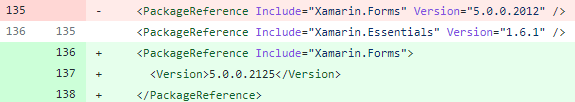
\includegraphics[width=15cm]{rys/gitchanges3.png}
			\caption{Modyfikacja NuGet Packages}
			\label{rys:Modyfikacja NuGet Packages}
		\end{center}
	\end{figure}
}

\newpage
\subsection{Dodanie oraz wystylizowanie elementów menu}

\textit
{
	Na początku należało utworzyć odpowiednie widoki aby stworzyć spójny szkielet aplikacji oraz stworzyć odpowiadające im modele widoków (rysunki 4.4 oraz 4.5).\\
	\begin{figure}[!htb]
		\begin{center}
			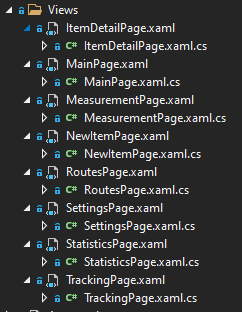
\includegraphics[width=7.5cm]{rys/gitchanges4.2.1.png}
			\caption{Szkielet widoków}
			\label{rys:Szkielet widoków}
		\end{center}
	\end{figure}
}

\textit
{
	\begin{figure}[!htb]
		\begin{center}
			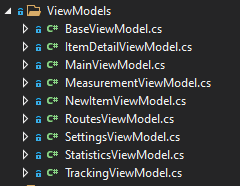
\includegraphics[width=7.5cm]{rys/gitchanges4.2.2.png}
			\caption{Szkielet modeli widoków}
			\label{rys:Szkielet modeli widoków}
		\end{center}
	\end{figure}
}

\newpage
\textit
{
	Następnym krokiem było ustawienie odpowiednich parametrów w celu połączenia poszczególnych widoków z ich modelami (zastosowano w tym celu dyrektywę Binding). Na rysunku 4.6 zaprezentowano jedną z takich modyfikacji.\\
	\begin{figure}[!htb]
		\begin{center}
			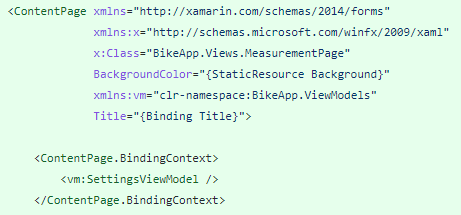
\includegraphics[width=15cm]{rys/gitchanges4.2.3.png}
			\caption{Łączenie ModelView z View}
			\label{rys:Łączenie ModelView z View}
		\end{center}
	\end{figure}
}

\newpage
\textit
{
	Kolejnym krokiem było ustawienie odpowiednich opcji FlyoutMenu (rysunek 4.7).\\
	\begin{figure}[!htb]
		\begin{center}
			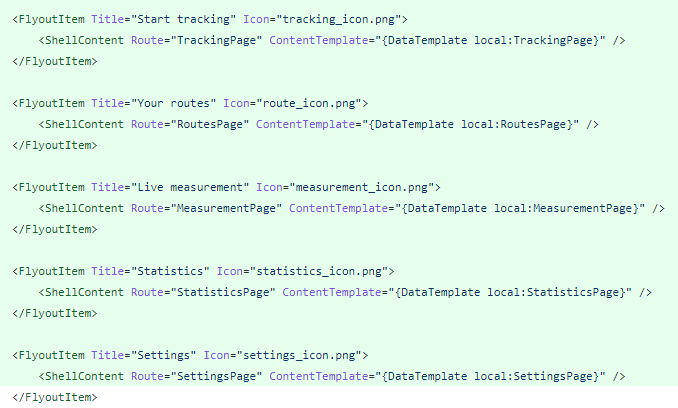
\includegraphics[width=15cm]{rys/gitchanges4.2.4.png}
			\caption{Dodanie opcji menu}
			\label{rys:Dodanie opcji menu}
		\end{center}
	\end{figure}
}

\newpage
\textit
{
	Po zakończeniu zostały stworzone oraz dodane odpowiednie ikony wraz z tytułami do każdego widoku (rysunki od 4.8 do 4.10)\\
	\begin{figure}[!htb]
		\begin{center}
			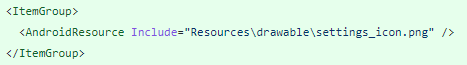
\includegraphics[width=15cm]{rys/gitchanges4.2.5.png}
			\caption{Dodanie ikon}
			\label{rys:Dodanie ikon}
		\end{center}
	\end{figure}
	\begin{figure}[!htb]
		\begin{center}
			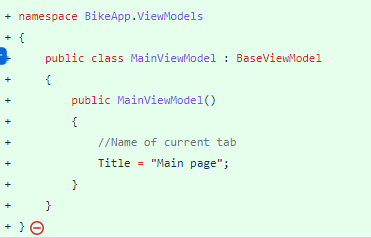
\includegraphics[width=10cm]{rys/gitchanges4.2.6.png}
			\caption{Dodanie tytułów widoków}
			\label{rys:Dodanie tytułów widoków}
		\end{center}
	\end{figure}
	\begin{figure}[!htb]
		\begin{center}
			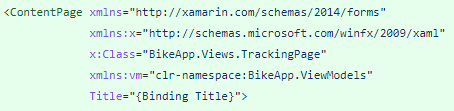
\includegraphics[width=15cm]{rys/gitchanges4.2.7.png}
			\caption{Dodanie styli}
			\label{rys:Dodanie styli}
		\end{center}
	\end{figure}
}

\newpage
\textit
{
	Ostatnim etapem, przedstawionym na rysunku 4.11, było wystylizowanie oraz poprawa ewentualnych błędów w kodzie.\\
	\begin{figure}[!htb]
		\begin{center}
			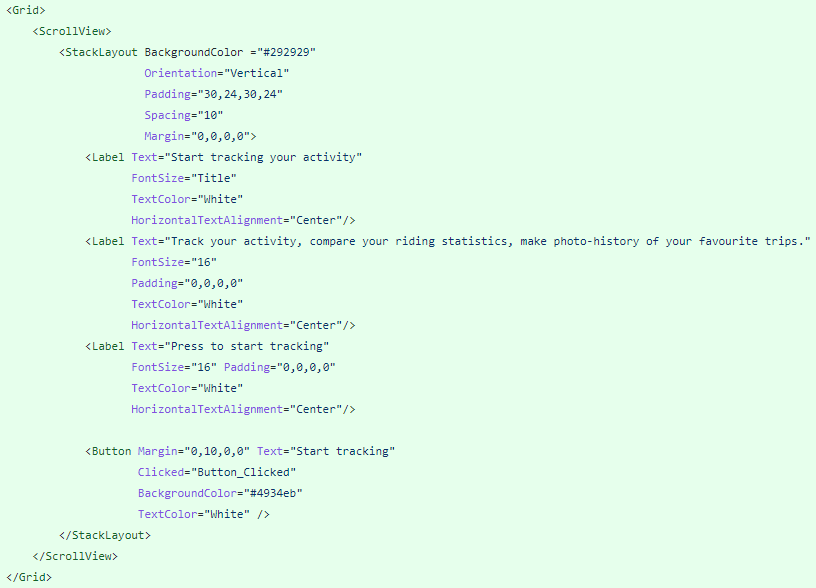
\includegraphics[width=15cm]{rys/gitchanges4.2.8.png}
			\caption{Finalizacja}
			\label{rys:Finalizacja}
		\end{center}
	\end{figure}
}

\newpage
\textit
{
	Efekt końcowy został zaprezentowany na rysunku 4.12.\\
	\begin{figure}[!htb]
		\begin{center}
			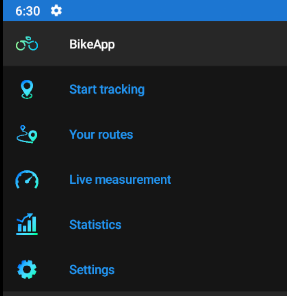
\includegraphics[width=10cm]{rys/gitchanges4.2.9.png}
			\caption{Wygląd menu po ukończeniu prac}
			\label{rys:Wygląd menu po ukończeniu prac}
		\end{center}
	\end{figure}
}

\newpage
\subsection{Dodanie motywu jasnego i ciemnego}

\textit
{
	Praca została rozpoczęta od utworzenia klas reprezentujących motywy i przechowujących odpowiadające im palety kolorów aplikacji (rysunki od 4.13 do 4.16).\\
	\begin{figure}[!htb]
		\begin{center}
			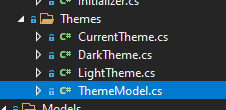
\includegraphics[width=7.5cm]{rys/gitchanges4.2.10.png}
			\caption{Układ klas motywów}
			\label{rys:Układ klas motywów}
		\end{center}
	\end{figure}
	\begin{figure}[!htb]
		\begin{center}
			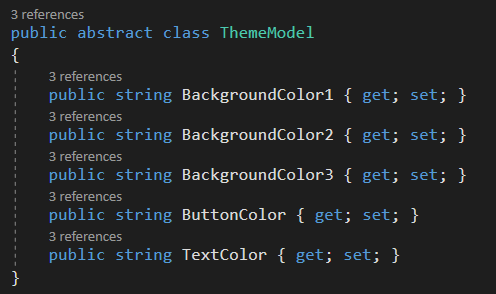
\includegraphics[width=10cm]{rys/gitchanges4.2.11.png}
			\caption{Kod abstrakcyjnej klasy bazowej}
			\label{rys:Kod abstrakcyjnej klasy bazowej}
		\end{center}
	\end{figure}
	\begin{figure}[!htb]
		\begin{center}
			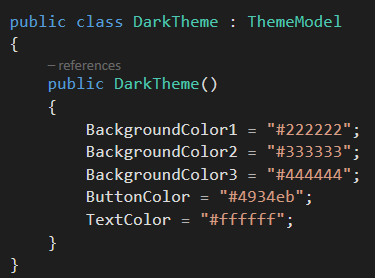
\includegraphics[width=10cm]{rys/gitchanges4.2.12.png}
			\caption{Przykładowy motyw dziedziczący po klasie bazowej}
			\label{rys:Przykładowy motyw}
		\end{center}
	\end{figure}
	\begin{figure}[!htb]
		\begin{center}
			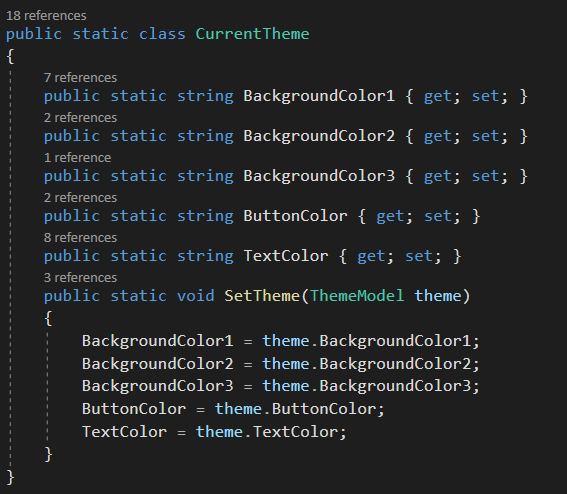
\includegraphics[width=10cm]{rys/gitchanges4.2.13.png}
			\caption{Klasa przechowująca aktualny motyw ustawiana na podstawie modelu abstrakcyjnego}
			\label{rys:Klasa przechowująca aktualny motyw}
		\end{center}
	\end{figure}
}
{
\newpage
	Motyw to klasa dziedzicząca po klasie bazowej z odpowiednio skonfigurowanym konstruktorem, dzięki takiej konstrukcji w razie potrzeby dodania kolejnych motywów nie ma potrzeby modyfikacji klasy głównej. Wystarczy dodać dowolną liczbę nowych motywów w postaci klas oraz przypisać obiekt nowo powstałej klasy w klasie inicjalizującej.
}

\textit
{
\newpage
	Kolejnym krokiem było stworzenie klasy przechowującej aktywny w danym momencie motyw (rysunek 4.17).\\
	\begin{figure}[!htb]
		\begin{center}
			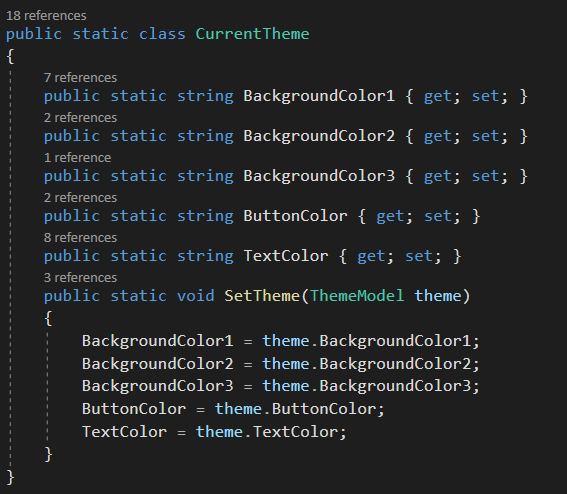
\includegraphics[width=10cm]{rys/gitchanges4.2.13.png}
			\caption{Klasa statyczna przechowująca motyw}
			\label{rys:Klasa statyczna}
		\end{center}
	\end{figure}
\\
	Następnie należało stworzyć metodę inicjalizującą ustawiającą motyw (rysunek 4.18) oraz wywołać ją w momencie ładowania aplikacji (rysunek 4.19).\\
	\begin{figure}[!htb]
		\begin{center}
			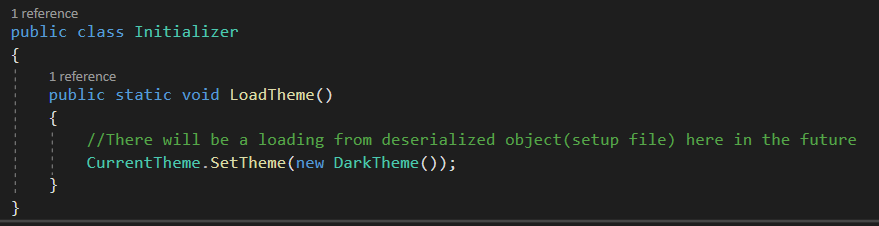
\includegraphics[width=15cm]{rys/gitchanges4.2.14.png}
			\caption{Klasa inicjalizująca}
			\label{rys:Klasa inicjalizująca}
		\end{center}
	\end{figure}
	\begin{figure}[!htb]
		\begin{center}
			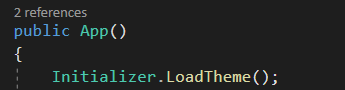
\includegraphics[width=10cm]{rys/gitchanges4.2.15.png}
			\caption{Klasa inicjalizująca - wywołanie}
			\label{rys:Klasa inicjalizująca - wywołanie}
		\end{center}
	\end{figure}
}

\textit
{
\newpage
	Następnie został stworzony mechanizm aktualizujący widok po każdym załadowaniu, przedstawiony na rysunku 4.20.\\
	\begin{figure}[!htb]
		\begin{center}
			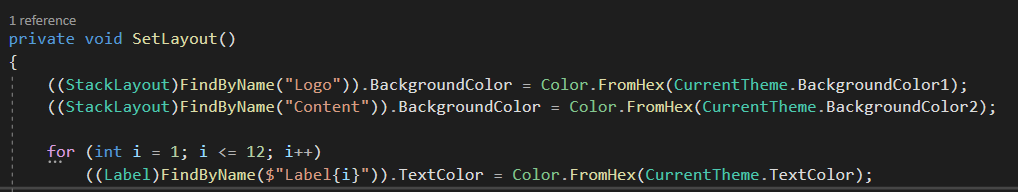
\includegraphics[width=15cm]{rys/gitchanges4.2.16.png}
			\caption{Aktualizacja widoku}
			\label{rys:Aktualizacja widoku}
		\end{center}
	\end{figure}
\\
	Na koniec do widoku dodano przełącznik sterujący zmianami motywu wraz z mechanizmem działania (rysunki 4.21 oraz 4.22).\\
	\begin{figure}[!htb]
		\begin{center}
			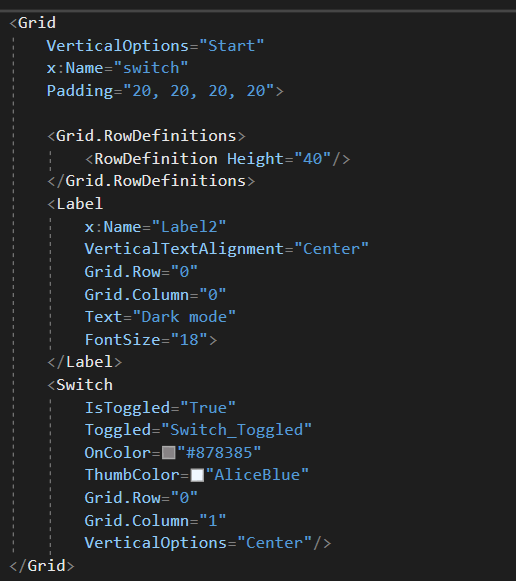
\includegraphics[width=10cm]{rys/gitchanges4.2.17.png}
			\caption{Kod XAML przełącznika}
			\label{rys:Kod XAML przełącznika}
		\end{center}
	\end{figure}
	\begin{figure}[!htb]
		\begin{center}
			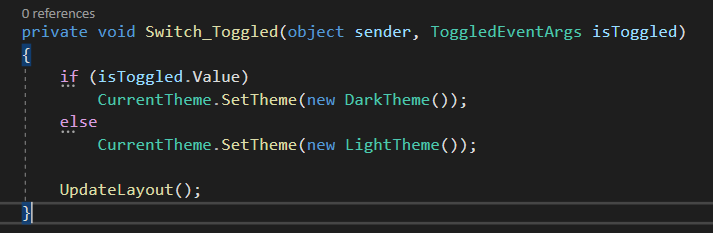
\includegraphics[width=15cm]{rys/gitchanges4.2.18.png}
			\caption{Mechanizm działania przełącznika}
			\label{rys:Mechanizm działania przełącznika}
		\end{center}
	\end{figure}
}

\newpage
\textit
{
	Rysunki 4.23 oraz 4.24 przedstawiają wygląd przełącznika oraz zmiany wyglądu całego widoku po jego użyciu.\\
	\begin{figure}[!htb]
		\begin{center}
			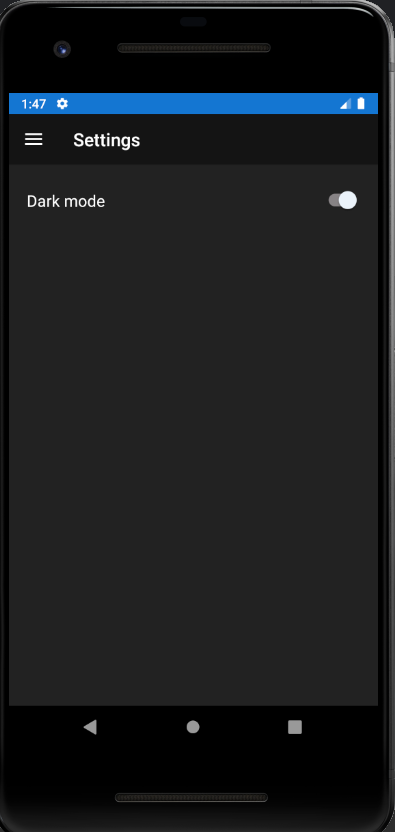
\includegraphics[width=6cm]{rys/gitchanges4.2.19.png}
			\caption{Włączenie trybu ciemnego}
			\label{rys:Włączenie trybu ciemnego}
		\end{center}
	\end{figure}
\\
	\begin{figure}[!htb]
		\begin{center}
			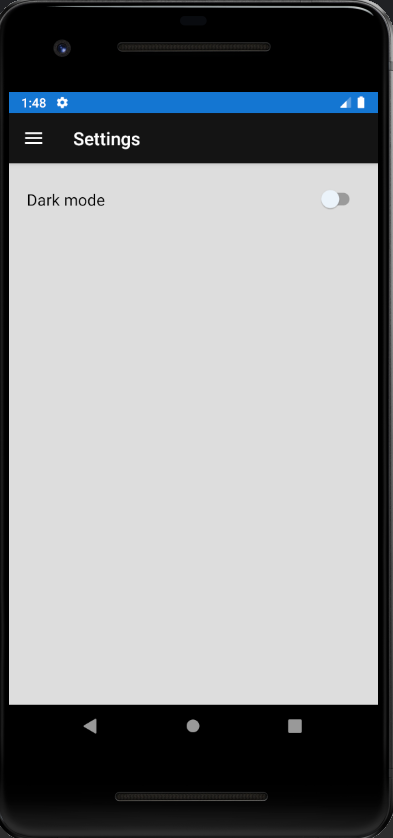
\includegraphics[width=6cm]{rys/gitchanges4.2.20.png}
			\caption{Wyłączenie trybu ciemnego}
			\label{rys:Wyłączenie trybu ciemnego}
		\end{center}
	\end{figure}
}



